\chapter{
  Introduction
 }\label{ch_intro}

\epigraph{\textit{It doesn't matter how beautiful your theory is,
    it doesn't matter how smart you are. \\
    If it doesn't agree with experiment, it's wrong.
    In that simple statement is the key to science.}}
{--- Richard P. Feynman}

``Particle Physics'' is the branch of physics which deals with the fundamental
particles and the interactions between them. Fundamental particles are the
subatomic particles which at our present level of understanding
are not made of other particles.
There are two types of fundamental particles ``matter'' and ``interaction''
particles. As the name suggests matter particles are the fundamental constituent
of matter and the interactions among them is governed by how they exchange interaction particles.
\gls{SM} of particle physics is the theory that classifies these fundamental
particles and describes three out of four fundamental
interaction forces; electromagnetic, weak, and strong.

This chapter briefly introduces the theory of \gls{SM}, Higgs mechanism,
spontaneous \gls{EWSB}, \gls{VBS}, and the motivation for the search of \gls{VBS}
in semileptonic decay channel \textit{ZV} with leptonic decay of \textit{Z},
and hadronic decay of \textit{V} (\textit{W}/\textit{Z}) to pair of quarks.

\section{
  Standard model
 }\label{ch_intro:standard-model}

In \gls{SM}, the matter particles are fermions, and
the interaction particles are bosons. \gls{SM} also includes
anti-fermions, which are fermions with equal mass but opposite sign of charge.
Figure~\ref{fig:standard-model-details} lists mass, electric charge,
and spin of fermions and bosons in the \gls{SM}.

Fermions obey Fermi-Dirac statistics and have half integer spin. They can be further
divided into leptons which have integral electric charge, and quarks which have
fractional electric charge. There are three generations of quarks and leptons
discovered to date, each generation only differing in mass.
In addition to the electric charge, quarks also have
three types of ``color'' charge (red, green and blue). Quarks cannot be isolated
because of ``color confinement'', which requires net color charge to be zero
for a free particle, for this reason we can only have certain composition
of quarks. Baryons (proton, neutrons, etc.) are made up of three quarks
each with different color charge,
and mesons (pions, kaons, etc.) are made of two quarks with color and anti-color charge.

Bosons obey Bose-Einstein statistics and have integral spin.
They are described by a local gauge theory and are also called gauge boson.
Photons are the interaction particle of electromagnetic force, they are massless
and only interact with charged particles. Gluons are the mediator of strong force
between the quarks, they are massless and carry color charge. \Wplusminus{} and \textit{Z}
are the vector bosons and mediator of weak force,
unlike photons and gluons they are massive. \Wplus{} and \Wminus{}
are antiparticles of each other, and \textit{Z} is its own antiparticle.
The last gauge boson, Higgs is a massive scalar boson with zero spin,
zero electric, and no color charge. Higgs boson is not a force carrier,
but rather explains why only some particles have mass.

The \gls{SM} is built in the framework of \gls{QFT}, in which particles
are excitation of the fields and interactions arise from local gauge
invariance. The \gls{SM} is a \( {SU(3)}_C \otimes {SU(2)}_L \otimes {U(1)}_Y\)
gauge theory, \( {U(1)}_Y \), \( {SU(2)}_L \), \( {SU(3)}_C \) are the gauge symmetries
of \gls{QED}, weak interaction and \gls{QCD} respectively, where the indices
stands for ``hypercharge'' (Y), ``left-handed'' (L) and ``color'' (C).

\begin{figure}[!ht]
  \centering
  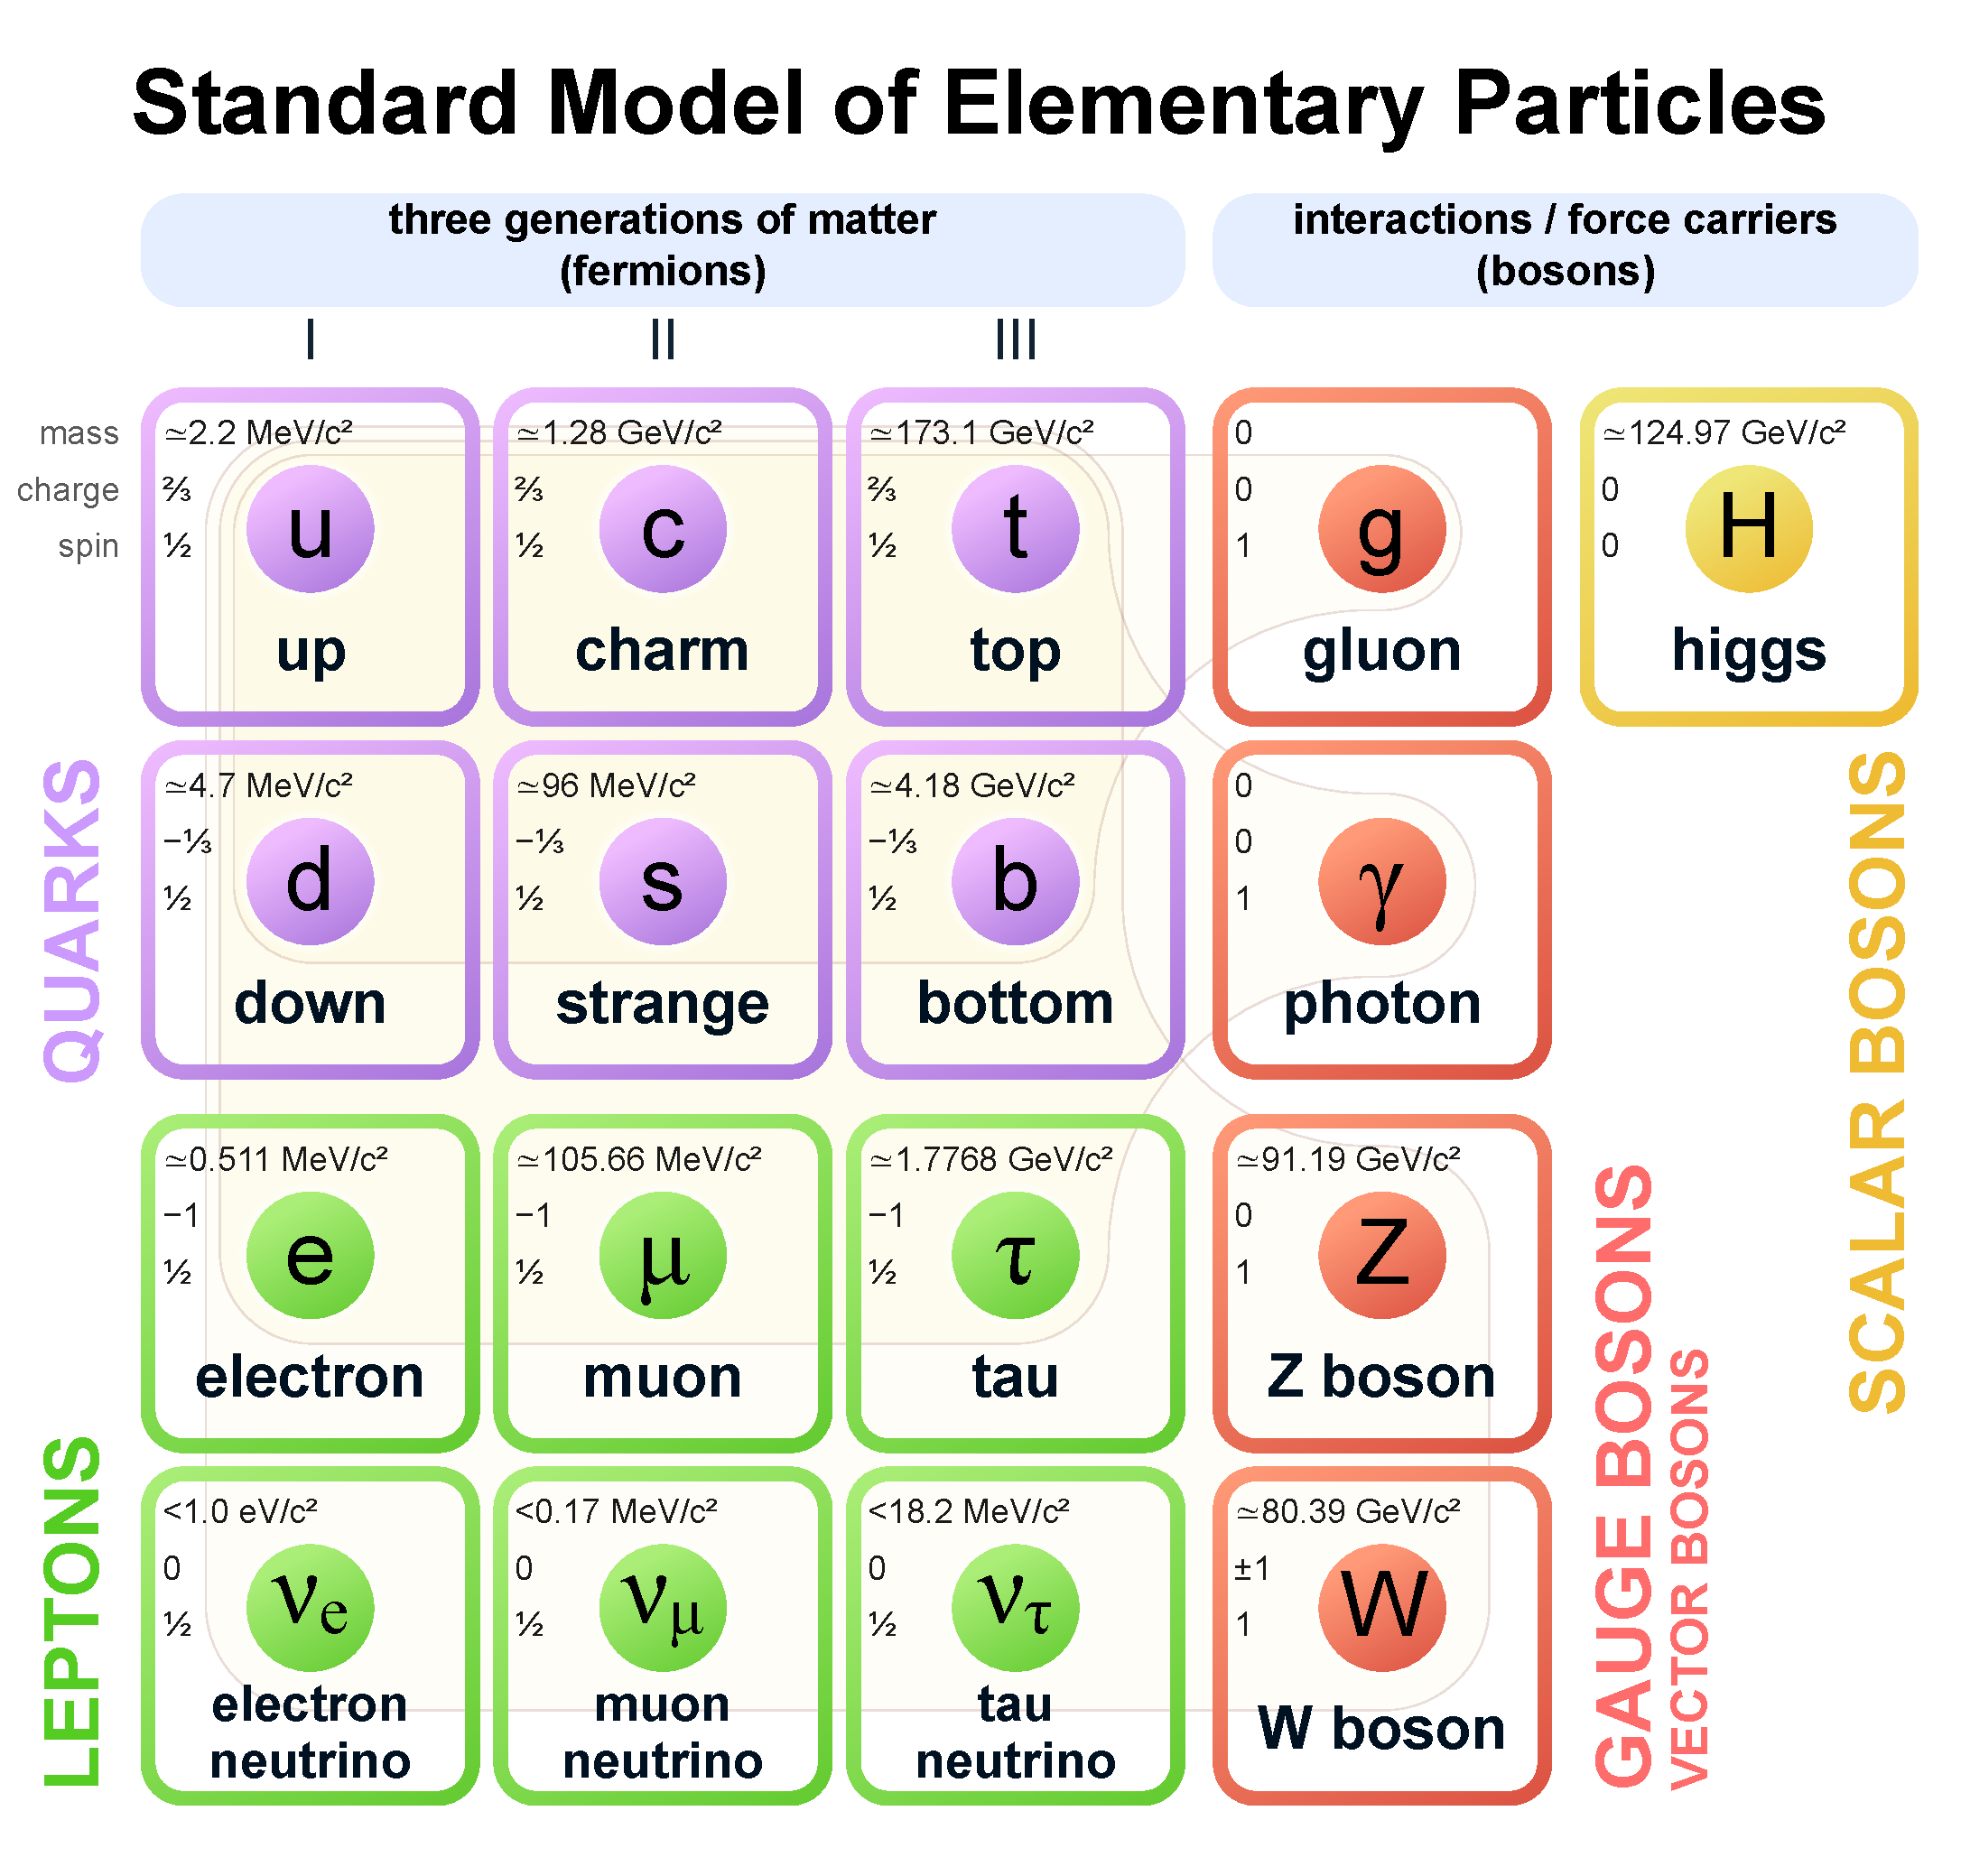
\includegraphics[width=0.8\textwidth]{figures/Standard_Model_of_Elementary_Particles.pdf}
  \caption[Standard model list of matter and interaction particles]%
  {Standard model list of matter and interaction particles~\cite{image-standard-model}}%
  \label{fig:standard-model-details}
\end{figure}

\subsection{
  Quantum Electrodynamics (QED)
}\label{ch_intro:qed}

\gls{QED} is a quantum field theory of electrodynamics, it describes
the interaction of photons to the charged fermions.
The \gls{QED} is local gauge invariant and symmetric with \( {U(1)}_{Q} \) symmetry group,
defined as,
%
\begin{align}
  {U(1)}_{Q} = \exp\left( { i Q \theta (x) } \right)
\end{align}

where \( \theta (x) \) is any spacetime function also called gauge parameter,
and \( Q \) is the coupling constant of photon field to the fermions
which is equivalent to the charge of fermion.

Under this transformation, fermion spinor \( \psi (x) \) and
four-potential \( A_{\mu} \) electromagnetic tensor will transform
as,
%
\begin{align}
  \psi (x) \rightarrow {U(1)}_{Q} \psi (x) \\
  A_{\mu} \rightarrow A_{\mu} - \frac{1}{e} \partial_{\mu} \theta
\end{align}

The general Lagrangian of \gls{QED} for fermions and their interaction
with photon field is given by,
%
\begin{equation}\label{eq:lag-qed}
  {\mathcal{L}}_{QED} = \bar{\psi} ( i {\gamma}^{\mu} {D}_{\mu} - m ) \psi
  - \frac{1}{4} {F}_{\mu \nu} {F}^{\mu \nu}
\end{equation}

where \( m \) is the mass of fermion,
\( {D}_{\mu} \) is the covariant derivative,
and \( {F}_{\mu \nu} \) is the electromagnetic field tensor defined as,
%
\begin{align}
  {D}_{\mu} = \partial_{\mu} + i Q A_{\mu} \\
  {F}_{\mu \nu} = \partial_{\mu} A_{\nu} - \partial_{\nu} A_{\mu}
\end{align}

\subsection{
  Quantum Chromodynamics (QCD)
}\label{ch_intro:qcd}

The strong interactions are represented by \( {SU(3)}_{C} \) gauge group, invariant
under transformations of color charge degree of freedom, based
on Yang-Mills theory~\cite{Yang-Mill:1954}. Since ``electrodynamics''
is the theory of electric charge, this theory of color (\textit{chromo} in Greek)
charge is called ``chromodynamics'', hence the name \glsfirst{QCD}.

A quark spinor in initial state can be represented as,
%
\begin{equation}
  \psi = \left( \begin{matrix}
    \psi_{red}  \\
    \psi_{blue} \\
    \psi_{green}
  \end{matrix} \right)
  = \left( \begin{matrix}
    \psi_{1} \\
    \psi_{2} \\
    \psi_{3}
  \end{matrix} \right)
\end{equation}

\( {SU(3)}_{C} \) is an exact symmetry, it means the difference between
colors cannot be measured experimentally, thus the color labels in quark spinor are arbitrary.
\( {SU(3)}_{C} \) transformation is defined as,
%
\begin{equation}
  {SU(3)}_{C} = \exp \left( {i \theta^{a}(x) \frac{\lambda^{a}}{2}} \right)
\end{equation}

where \( \lambda^{a} \) for \( a = 1,\ldots,8\),
are the Gell-Mann matrices, and \( \theta^{a}(x) \) are any gauge parameters.
These eight generators of symmetry corresponds to eight gauge vector boson gluons.

Similar to \gls{QED}, the covariant derivative for \gls{QCD} can be formed as,
%
\begin{equation}
  D_{\mu} = \partial_{\mu} + i g_s \frac{\lambda^{a}}{2} G_{\mu}^{a}
\end{equation}

where \( g_s \) is the coupling constant of gluon to the quarks,
and \( G_{\mu}^{a} \) are the eight gauge fields corresponding to gluons.

The corresponding field strength tensor in \gls{QCD} can be formed as,
%
\begin{equation}
  F_{\mu \nu}^{a} = \partial_{\mu} G_{\nu}^{a} - \partial_{\nu} G_{\mu}^{a}
  - g_s f^{abc} G_{\mu}^{b} G_{\nu}^{c}
\end{equation}

where \( f^{abc} \) are the structure constants of \( {SU(3)}_{C} \)
which satisfy \( [\lambda^{a}, \lambda^{b}] = i f^{abc} \lambda^{c} \) relation.

The full Lagrangian for \gls{QCD} can now be constructed as,
%
\begin{equation}
  {\mathcal{L}}_{QCD} = {\bar{\psi}}^{i}
  ( i {\gamma}^{\mu} {{D}_{\mu}}^{ij} - m \delta^{ij} )\psi^{j}
  - \frac{1}{4} {F}_{\mu \nu}^{a} {F}^{a \mu \nu}
\end{equation}

for mass \( m \), indices \( i \) and \( j \) runs from 1 to 3.

The main difference of gluon field with respect to photon field is
the presence of third term in
field strength tensor which allows triplet and quartic
self coupling of gluons.

\subsection{
  Electroweak Theory
}\label{ch_intro:ew}

Weak interaction occurs for all the fermions via the exchange of
massive vector bosons \Wplusminus{}, \textit{Z}.
Since the unification of electromagnetic
and weak interaction into \gls{EW} interaction by
Glashow, Weinberg, and Salam~\cite{Glashow1959,Weinberg1967,Salam1959},
the weak interaction is better understood in terms of \gls{EW} theory.

Weak interaction only couples to left-handed fermions and it is same
whether the fermion is charged or not. The underlying gauge group of
\gls{EW} interaction is \( {SU(2)}_{L} \otimes {U(1)}_{Y} \) and
has two transformations one for the left-handed doublet
\( L \) and the right handed singlet fermions \( \psi_R \) which are defined as,
%
\begin{align}
  {SU(2)}_{L} \otimes {U(1)}_{Y} & =
  \exp \left( {i \theta^{a}(x) \frac{\sigma^a}{2}} + {i \theta(x) \frac{Y}{2}} \right)
  , \quad (doublet)                                                                \\
                                 & = \exp \left( {i \theta(x) \frac{Y}{2}} \right)
  , \quad (singlet)
\end{align}

where \( Y \) is the hypercharge (linear combination of electric charge and weak
isospin component), and \( \sigma^{a} \) for \( a = 1,2,3 \)
are the Pauli spin matrices generator of \( SU(2) \) symmetry. Left-handed
fermion \( L \) doublets are,
%
\begin{equation}
  L = \left(\begin{matrix}
    \nu_e \\
    e_L
  \end{matrix}\right) ,
  \left(\begin{matrix}
    \nu_\mu \\
    \mu_L
  \end{matrix}\right) ,
  \left(\begin{matrix}
    \nu_\tau \\
    \tau_L
  \end{matrix}\right) ,
  \left(\begin{matrix}
    u_L \\
    d_L
  \end{matrix}\right) ,
  \left(\begin{matrix}
    c_L \\
    s_L
  \end{matrix}\right) ,
  \left(\begin{matrix}
    t_L \\
    b_L
  \end{matrix}\right)
\end{equation}

and right-handed singlets are,
%
\begin{equation}
  \psi_R = e_R, \mu_R, \tau_R, u_R, d_R, c_R, s_R, t_R, b_R
\end{equation}

The covariant
derivative of \gls{EW} is then,
%
\begin{align} \label{eq:ew-dmu}
  D_{\mu} L      & = \left( \partial_{\mu} + i g_w \frac{\sigma^{a}}{2} W^{a}_{\mu} + i g \frac{Y}{2} B_{\mu} \right) L \\
  D_{\mu} \psi_R & = \left( \partial_{\mu} + i g \frac{Y}{2} B_{\mu} \right) \psi_R
\end{align}

where \( W^{a}_{\mu} \) and \( B_{\mu} \) are the gauge fields. The \gls{EW}
Lagrangian can now written as,
%
\begin{align}
  \mathcal{L}_{EW} = i \bar{L} \gamma^{\mu} D_{\mu} L
  + i \bar{\psi}_R \gamma^{\mu} D_{\mu} \psi_R
  - \frac{1}{4} {W}_{\mu \nu}^{a} {W}^{a \mu \nu}
  - \frac{1}{4} {B}_{\mu \nu} {B}^{\mu \nu}
\end{align}

where \( B_{\mu \nu} \) and \( W^{a}_{\mu \nu} \) are fields strength,
defined as,
%
\begin{align}
  B_{\mu \nu }    & = \partial_{\mu} B_{\nu} - \partial_{\nu} B_{\mu}         \\
  W_{\mu \nu}^{a} & = \partial_{\mu} W_{\nu}^{a} - \partial_{\nu} W_{\mu}^{a}
  - g_w \epsilon^{abc} W_{\mu}^{b} W_{\nu}^{c}
\end{align}

the linear combination of \( B_{\mu} \) and \( W_{\mu} \) gauge field, with a weak mixing
angle \( \theta_w \) gives 4 vectors boson \Wplus, \Wminus, \textit{Z}, and \( \gamma \) of \gls{SM},
%
\begin{align}
  W^{\pm}_{\mu} & = \frac{1}{\sqrt{2}} \left( W^{1}_{\mu} \mp W^{2}_{\mu} \right) \\
  Z_{\mu}       & = \cos \theta_w W^{3}_{\mu} - \sin \theta_w B_{\mu}             \\
  A_{\mu}       & = \sin \theta_w W^{3}_{\mu} + \cos \theta_w B_{\mu}             \\
  \tan \theta_w & = g/g_{w}
\end{align}

Similar to \gls{QCD}, the presence of third term in field strength tensor
allows the self triple (\textit{WWZ}, \textit{WW}\( \gamma \)) and quartic (\textit{WWWW},
\textit{WWZZ}, \textit{WWZ}\( \gamma \),
\textit{WW}\( \gamma \gamma \)) couplings.

\subsection{
  Electroweak Symmetry Breaking and Higgs Mechanism
}\label{ch_intro:ewsb}

\textit{Spontaneous symmetry breaking} is the phenomena which explains
why the ground state is not invariant under the symmetry
of the Lagrangian. ``Spontaneous'' means that the symmetry
breaking is not done by external agent but rather by Lagrangian itself
in ground state.

The \gls{EW} theory unifies weak interaction and \gls{QED} but the
gauge boson in \gls{EW} theory are all massless, if we were to add mass
terms like \( - m^{2} W_{\mu} W^{\mu} \) by hand, it will no longer
be gauge invariant. The solution to this, without breaking gauge invariance,
is spontaneous symmetry breaking, but this requires addition of new scalar
field called Higgs field via \gls{BEH}~\cite{Englert1964,Higgs1964}, and this
symmetry breaking is known as \glsfirst{EWSB}.

\gls{BEH} introduces a complex scalar field as \( {SU(2)}_L \)
doublet with non-zero \gls{VEV},
%
\begin{equation}
  \phi = \left( \begin{matrix}
      \phi^{+} \\
      \phi^{0}
    \end{matrix} \right)
  = \frac{1}{\sqrt{2}}
  \left( \begin{matrix}
      \phi^{1} + i \phi^{2} \\
      \phi^{3} + i \phi^{3}
    \end{matrix} \right)
\end{equation}

and \gls{BEH} Lagrangian is,
%
\begin{equation}
  \mathcal{L}_{BEH} = {| D_{\mu} \phi |}^{2} - V(\phi)
\end{equation}

where \( D_{\mu} \) is same as \gls{EW} covariant derivate
in Equation~\ref{eq:ew-dmu}, and \( V(\phi) \) is,
%
\begin{equation}
  V(\phi) = \mu^{2} |\phi|^{2} + {\lambda (|\phi|^{2})}^{2}
\end{equation}

the parameter \( \lambda \) is required to be positive,
for \( \mu^2 > 0\) the minima is at 0, which is not an interesting case,
but for \( \mu^2 < 0\) vacuum state energy is given by,
%
\begin{equation}
  \phi^{\dagger} \phi = - \frac{\mu^{2}}{2 \lambda}
\end{equation}

by the choice of non-zero \gls{VEV} \( v \), scalar field can be parameterized as,
%
\begin{align}
  v        & = \sqrt{\frac{- \mu^2}{\lambda}}                 \\
  \phi (x) & = \frac{1}{\sqrt{2}} \left( \begin{matrix}
                                             0 \\
                                             h (x) + v
                                           \end{matrix} \right)
\end{align}

where \( h(x) \) is the Higgs field and \gls{BEH} spontaneously breaks electroweak symmetry,
%
\begin{equation}
  {SU(2)}_L \otimes {U(1)}_Y \rightarrow {U(1)}_{EM}
\end{equation}

Visually the Higgs potential is shown in Figure~\ref{fig:higgs-potential}. The ball position
at the center represents unbroken symmetry, and at the minima represents spontaneous
broken symmetry in the ground state of potential.
%
\begin{figure}[!ht]
  \centering
  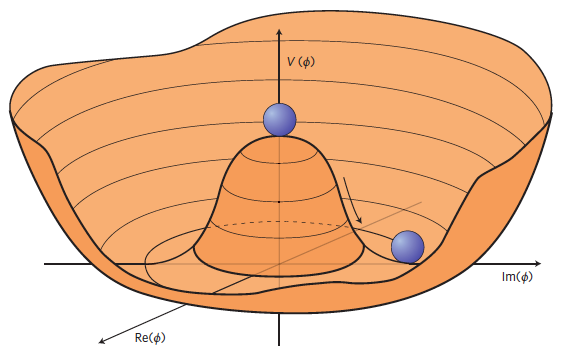
\includegraphics[width=0.7\textwidth]{figures/higgspotential.png}
  \caption[3D representation of Higgs potential]%
  {3D representation Higgs potential~\cite{image-higgs-potential}.}%
  \label{fig:higgs-potential}
\end{figure}

After \gls{EWSB}, the \gls{BEH} Lagrangian contains the following mass terms,
%
\begin{align}
  m^{2}_{W} W^{+}_{\mu} W^{- \mu}, \quad
  m^{2}{Z} Z_{\mu}Z^{\mu}, \quad m^{2} h^{2}
\end{align}

and gauge fields,
%
\begin{align}
  - \frac{1}{4} A_{\mu \nu} A^{\mu \nu}, \quad
  - \frac{1}{4} W^{+}_{\mu \nu} W^{- \mu \nu}, \quad
  - \frac{1}{4} Z_{\mu \nu} Z^{\mu \nu}, \quad
  - \frac{1}{4} {(\partial_{\mu} h)} {(\partial^{\mu} h)}
\end{align}

thus explaining existence of three massive vector boson (\Wplusminus{}, Z), one massless
vector boson (\( \gamma \)), and one massive scalar boson Higgs (H).

With experimentally measured value of \gls{VEV} \( v \) approximately 246 \GeV{},
The masses of bosons can be written in terms of \( v \) as,
%
\begin{align}
  m_A = 0, \quad
  m_W = \frac{g_{W} v}{2}, \quad
  m_Z = \frac{\sqrt{g^{2}_{W} + g^{2}} v }{2}, \quad
  m_H = \sqrt{2\lambda} v
\end{align}

\section{
  Vector Boson Scattering
 }\label{ch_intro:vbs}

The \glsfirst{VBS} is a key process to experimentally study the nature of
\gls{EWSB} mechanism, because massive vector boson at high energy
scattering can probe \gls{EW} theory at \TeV{} scale.
This section describes the motivation behind studying \gls{VBS}, and
the topology of scattering of \textit{ZV} channel studied in this dissertation.

\subsection{Motivation}

A massless spin-1 boson can exists in two transverse polarization as,
%
\begin{equation}
  \varepsilon^{\mu}_{\pm} = \mp \frac{1}{\sqrt{2}} (0, 1, \pm i, 0)
\end{equation}

and massive vector bosons can also exists in one longitudinal polarization,
%
\begin{equation}
  \varepsilon^{\mu}_{L} = \frac{1}{m} (p_z, 0, 0 , E)
\end{equation}

This means the longitudinal polarized \gls{VBS} cross-section will scale as \( E/m \),
whereas the scattering cross-section of transverse polarized boson remains constant.
Figure~\ref{fig:vbs-at-high-energies} shows the cross-section
of longitudinal polarized \gls{VBS} \( V_L V_L \to V_L V_L\)
from low to high energies. Perturbatively, the cross-section of
longitudinal polarized \gls{VBS} will scale with center of mass energy
\( \sqrt{s} \) and eventually unitarity is violated at
\( \approx 1.2 \TeV{} \) scale~\cite{Lee1977,Lee1977a}.
Figure~\ref{fig:vbs-at-high-energies} also shows
how the existence of light Higgs boson and
inclusion of Higgs to vector boson coupling diagrams in longitudinal
polarized \gls{VBS} can restore unitarity,
and any deviation from \gls{SM} Higgs to vector
bosons coupling will be visible in such a di-boson spectrum.

\begin{figure}[!ht]
  \centering
  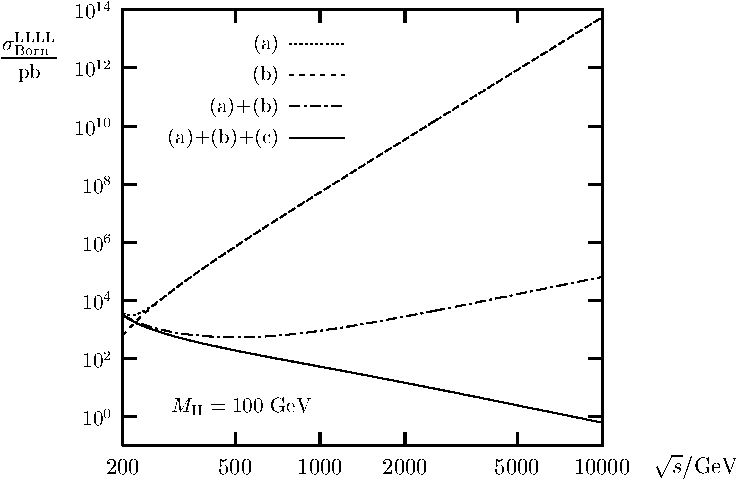
\includegraphics[width=0.6\textwidth]{figures/unitarity.pdf}
  \caption[The cross-sections for longitudinal polarized \gls{VBS} involving three
    and four-boson coupling with and without Higgs coupling included.]%
  {The cross-sections for longitudinal polarized \gls{VBS} involving three
    and four-boson coupling with and without Higgs coupling diagram included.
    (a) is for the diagrams with three-boson coupling,
    (b) is for diagrams with four-boson coupling, and (c) is for diagrams
    with Higgs to vector boson coupling.~\cite{Denner1997}}%
  \label{fig:vbs-at-high-energies}
\end{figure}


Thus \gls{VBS} measurement serves the two-fold purpose of
doing precise measurements of the Higgs coupling to vector bosons
at higher energy scales,
and providing a framework to test for anomalous quartic gauge
couplings in the \gls{SM}.


\subsection{
  Topology of VBS in Semileptonic \textit{ZV} Final State
}

As discussed in previous section, \gls{VBS} in \gls{SM} can
proceed via exchange of vector boson, Higgs
boson, or quartic gauge coupling of four vector bosons.
Figure~\ref{fig:feynman-vbs-general},~\ref{fig:feynman-vbs-blob}
shows tree level Feynman diagrams for \gls{VBS} process.

\begin{figure}[!ht]
  \centering
  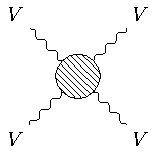
\includegraphics[width=0.3\textwidth]{figures/feyn_vbs_general.pdf}
  \caption[Tree level Feynman diagram of \textit{VV} \gls{VBS}]%
  {Tree level Feynman diagram of \textit{VV} \gls{VBS},
    where \textit{V} can be \Wplusminus{}, \textit{Z}, or \( \gamma \)}%
  \label{fig:feynman-vbs-general}
\end{figure}

\begin{figure}[!ht]
  \centering
  \begin{minipage}{0.23\textwidth}
    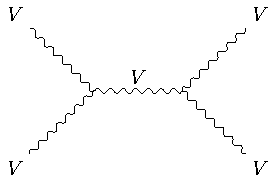
\includegraphics[width=\textwidth]{figures/feyn_vbs_2.pdf}
  \end{minipage}%
  \begin{minipage}{0.18\textwidth}
    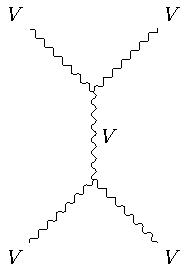
\includegraphics[width=\textwidth]{figures/feyn_vbs_4.pdf}
  \end{minipage}%
  \begin{minipage}{0.23\textwidth}
    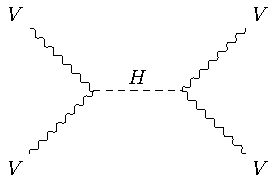
\includegraphics[width=\textwidth]{figures/feyn_vbs_3.pdf}
  \end{minipage}%
  \begin{minipage}{0.18\textwidth}
    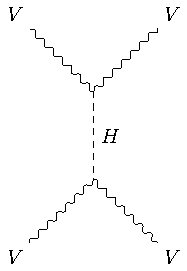
\includegraphics[width=\textwidth]{figures/feyn_vbs_5.pdf}
  \end{minipage}%
  \begin{minipage}{0.16\textwidth}
    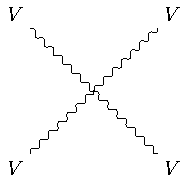
\includegraphics[width=\textwidth]{figures/feyn_vbs_1.pdf}
  \end{minipage}
  \caption[Tree level processes that can happen in scattering represented by blob
    in \textit{VV} VBS]%
  {Tree level processes that can happen in scattering represented by blob
    in \textit{VV} VBS, starting from s and t-channel exchange of
    vector boson, Higgs boson, and the last one is quartic
    coupling of vector bosons.
  }%
  \label{fig:feynman-vbs-blob}
\end{figure}

In proton-proton collisions, the actual interaction happens
with the constituent quarks. For \gls{VBS} to occur, the incoming
(colliding) quarks have to radiate vector boson, then the scattering
process between those vector boson can proceed via exchange of vector
boson, Higgs boson, or quartic coupling. The tree level Feynman
diagram of a \textit{ZV} VBS process in proton-proton
collision is shown in Figure~\ref{fig:feynman-vbs}.

The outgoing quarks are a key signature of \gls{VBS} in hadron collider
experiments because they will have large pseudorapidity\footnote{
  defined as \(\eta = - \ln[\tan \theta/2]\), where \(\theta \) is angle
  between the \(z\)-axis and the beam-axis. }
difference between
them, corresponding to a large invariant mass of outgoing quark pair.
These outgoing quarks are first identified
and tagged to filter out most of the \gls{QCD} background.

\begin{figure}[!ht]
  \centering
  \begin{minipage}{0.5\textwidth}
    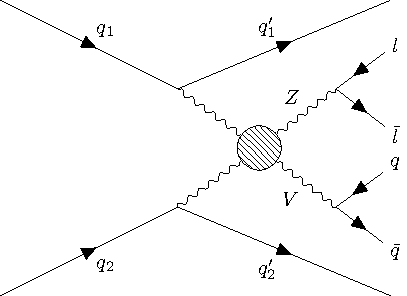
\includegraphics[width=\textwidth]{figures/feyn_vbs_0.pdf}
    \vspace{5pt}
  \end{minipage}
  \caption[Tree level Feynman diagram of \textit{ZV} VBS process at LHC]%
  {Tree level Feynman diagram of \textit{ZV} VBS process at LHC\@. The diagram
    shows the production of two vector boson being radiated from incoming
    quarks, in final state after scattering (blob), \textit{Z} decays
    to pair of leptons, \textit{V} (\textit{W}/\textit{Z}) decays to pair of quarks,
    and plus two outgoing quarks.
  }%
  \label{fig:feynman-vbs}
\end{figure}

The type of leptonically decaying
vector boson can be determined from the number of leptons in final state i.e.
whether it was \textit{W} (1 lepton + 1 neutrino) or \textit{Z} (2 leptons).
But given the hadronic activity
in the proton-proton collisions, it is challenging
to determine the type of hadronically decaying vector
boson and is generally denoted by \textit{V}.

Depending upon the decay channel of vector bosons, \gls{VBS} can
be categorized into fully leptonic or hadronic, or semileptonic channels.
The fully leptonic channel has the cleanest signal, but the signal yield
is also lower. The fully hadronic channel has the highest
signal yield but also have large background because of hadronic activity
in the final state.
The semileptonic final state sits in-between these two channels,
with cleaner boson reconstruction from leptons, and larger yields
from hadronically decaying boson.

Out of two channels in the semileptonic, \textit{WV} and \textit{ZV},
\textit{WV} has been studied and published by the \gls{CMS}~\cite{vbs-wv-cms-2021}.
Anomalous quartic gauge coupling limits derived using semileptonic
channels with 2016 data of the \gls{CMS} have also been published~\cite{wv-vbs-aqgc}.

This analysis looks for the \gls{VBS} signature with \textit{ZV} in final state
with the \textit{Z} decaying to two \gls{OSSF} leptons, and \textit{V} decaying to a pair
of quarks in association with two outgoing quarks. Chapter~\ref{ch_cms}
describes the proton-proton collision data used in this analysis and how
various subdetectors of the \gls{CMS} experiment work to capture the
event information. Then in Chapter~\ref{ch_reco} the particle
reconstruction and event simulations are discussed. In the
Chapter~\ref{ch_vbs} the object and events selection
used are listed, the signal vs background classifier developed
is described, and finally the measurement of signal significance is discussed.
